\documentclass[a4paper,11pt]{article}


\usepackage[utf8]{inputenc} %damit man auch Umlaute eingeben kann
\usepackage[bitstream-charter]{mathdesign} % Charter als Standardschriftart
\usepackage[T1]{fontenc} %damit Umlaute bei einer pdf-Suche auch erkannt werden
\usepackage[scaled=.82]{DejaVuSansMono} % DejaVuSansMono als Code-Schriftart
\usepackage{graphicx} %für Grafiken der Formate jpg, png, pdf
\usepackage{amsfonts,amsmath} %Verwendung von Mathematik-Schriftarten
\usepackage{url} %für die gute Darstellung von Internet-Links
\usepackage{float} % um Abbildung wirklich genau dort zu platzieren
% \usepackage[ngerman]{babel} %deutsches Sprachpaket
\usepackage[ngerman,english]{babel} %deutsches Sprachpaket
\usepackage[round]{natbib} %für vereinfachte:wen/Querverweise
\usepackage{paracol}
\usepackage{tikz} %für tikz-Grafiken
\usepackage{quoting}
\usepackage{subfigure}
\usepackage{pgfplots}
\usepackage{capt-of}
\usepackage{listings} % für Quelltext mit Syntax-Highlighting
\usepackage[colorlinks=true, allcolors=blue]{hyperref}
\usepackage{enumerate}
\setlength\parindent{0pt}
\pgfplotsset{width=0.8\textwidth,compat=1.9}
\lstset{
	backgroundcolor=\color[HTML]{E8F2F2},
	keywordstyle=\color{blue},
    breaklines=true,
	basicstyle=\small\ttfamily,
	commentstyle=\color{brown},
	numbers=left,
	%numberstyle=\tiny,
	%frame=leftline,
	%xleftmargin=.04\textwidth,
	inputencoding=utf8,
	extendedchars=true,
	literate={ä}{{\"a}}1 {à}{{\`a}}1 {ö}{{\"o}}1 {ü}{{\"u}}1 {è}{{\`e}}1 {é}{{\'e}}1}
\lstnewenvironment{pycode}[1][] % für abgesetzten rust code
{\lstset{
	language=Python,
	backgroundcolor=\color[HTML]{E8F2F2},
    breaklines=ture,
	basicstyle=\small\ttfamily,
	keywordstyle=\color{blue},
	commentstyle=\color{brown},
	numbers=left,
	%numberstyle=\tiny,
	%xleftmargin=.04\textwidth,
	%frame=leftline,
	inputencoding=utf8,
	extendedchars=true,
	literate={ä}{{\"a}}1 {à}{{\`a}}1 {ö}{{\"o}}1 {ü}{{\"u}}1 {è}{{\`e}}1 {é}{{\'e}}1,
	#1}}{}
\providecommand{\pyinline}{\lstinline[language=Python,basicstyle=\ttfamily,keywordstyle=\color{blue},commentstyle=\color{brown}, literate={ä}{{\"a}}1 {à}{{\`a}}1 {ö}{{\"o}}1 {ü}{{\"u}}1 {è}{{\`e}}1 {é}{{\'e}}1]} % für Inline-C++ Code
\title{Bandstop filters and }
\author{Gian Laager and Sebastian Rast}
\begin{document}

\maketitle

\section{Introduction}

\subsection{Goal}
\subsection{Hypothesis}

A LC circuit has the ability to oscillate on is own i.e. it can produce a current that looks like some kind of sin-wave over time. This feature is provided by the interaction of a coil and a capacitor. The circuit has to be assembled according to the circuit in fig. \ref{fig:lc}.
\subsection{How does a LC circuit work?}
\section{Theoretical Background}

\begin{figure}[!ht]
    \centering
    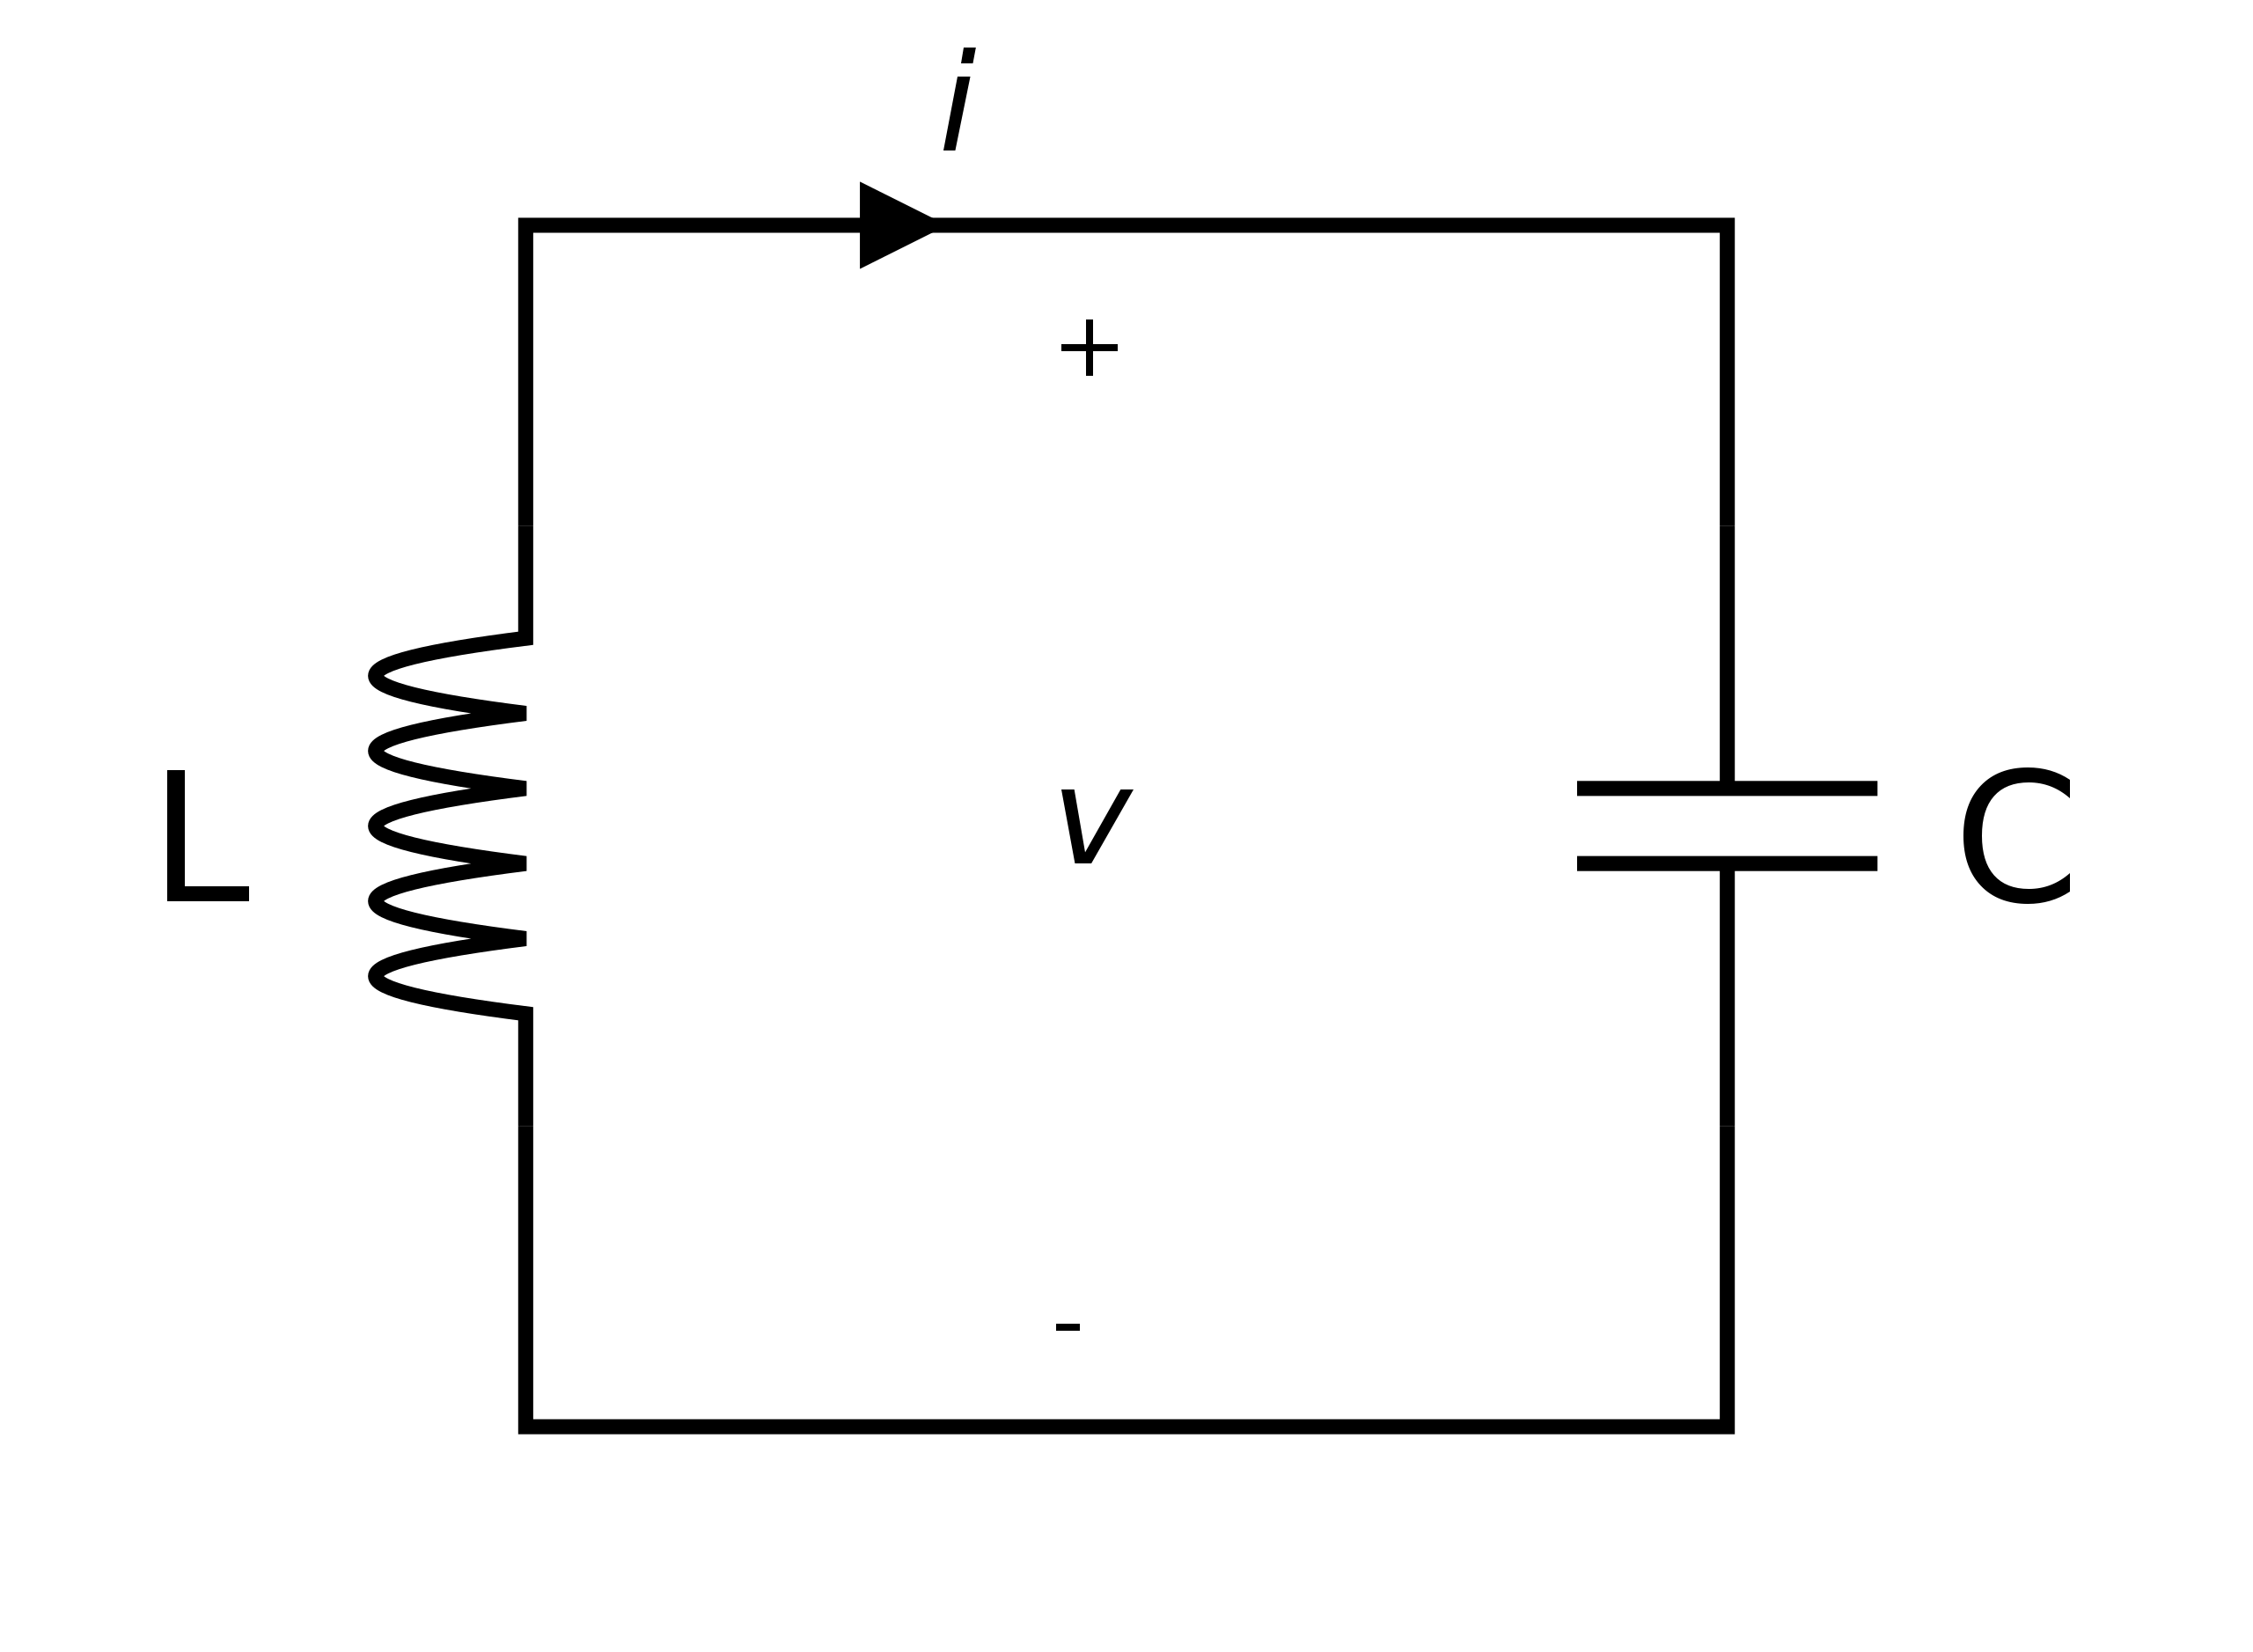
\includegraphics[width=0.5\textwidth]{images/2560px-LC_parallel_simple.svg.png}
    \caption{Schematic of a LC circuit}
    \label{fig:lc}
\end{figure}

In principle a LC circuit works as following:
\begin{enumerate}[I.]
    \item At the beginning the capacitor is charged and a voltage can be measured over the capacitor. All the energy is stored in the capacitor.
    \item Because of the voltage, current flows from the capacitor to the inductor and the inductor is charged.
    \item The charging of the inductor leads to a magnetic field produced by the coil. According to the Lenz rule this magnetic field acts against the flowing current. Thus the increase of the current happens slowly at the beginning. At the end though, the current increases with the magnetic field until a maximum is reached. At this time the capacitor is fully discharged and the energy is stored in the inductor.
    \item After the current has reached its maximum it will slowly decrease and the magnetic field is dissipated. Hence no voltage is applied to the inductor. 
    \item The same cycle starts again just with a negative voltage.
    \item The current flows on and charges the capacitor until all of the energy is transferred to the capacitor. 

\end{enumerate}
\subsection{Bandstop filter}
A bandstop filter has the ability to pass almost all frequencies but filter very specific frequencies (= bands) (see fig.\ref{fig:bsf}). Bandstop filters are used in various applications as for example guitar amplifiers or the Raman spectroscopy.
\begin{figure}[!ht]

    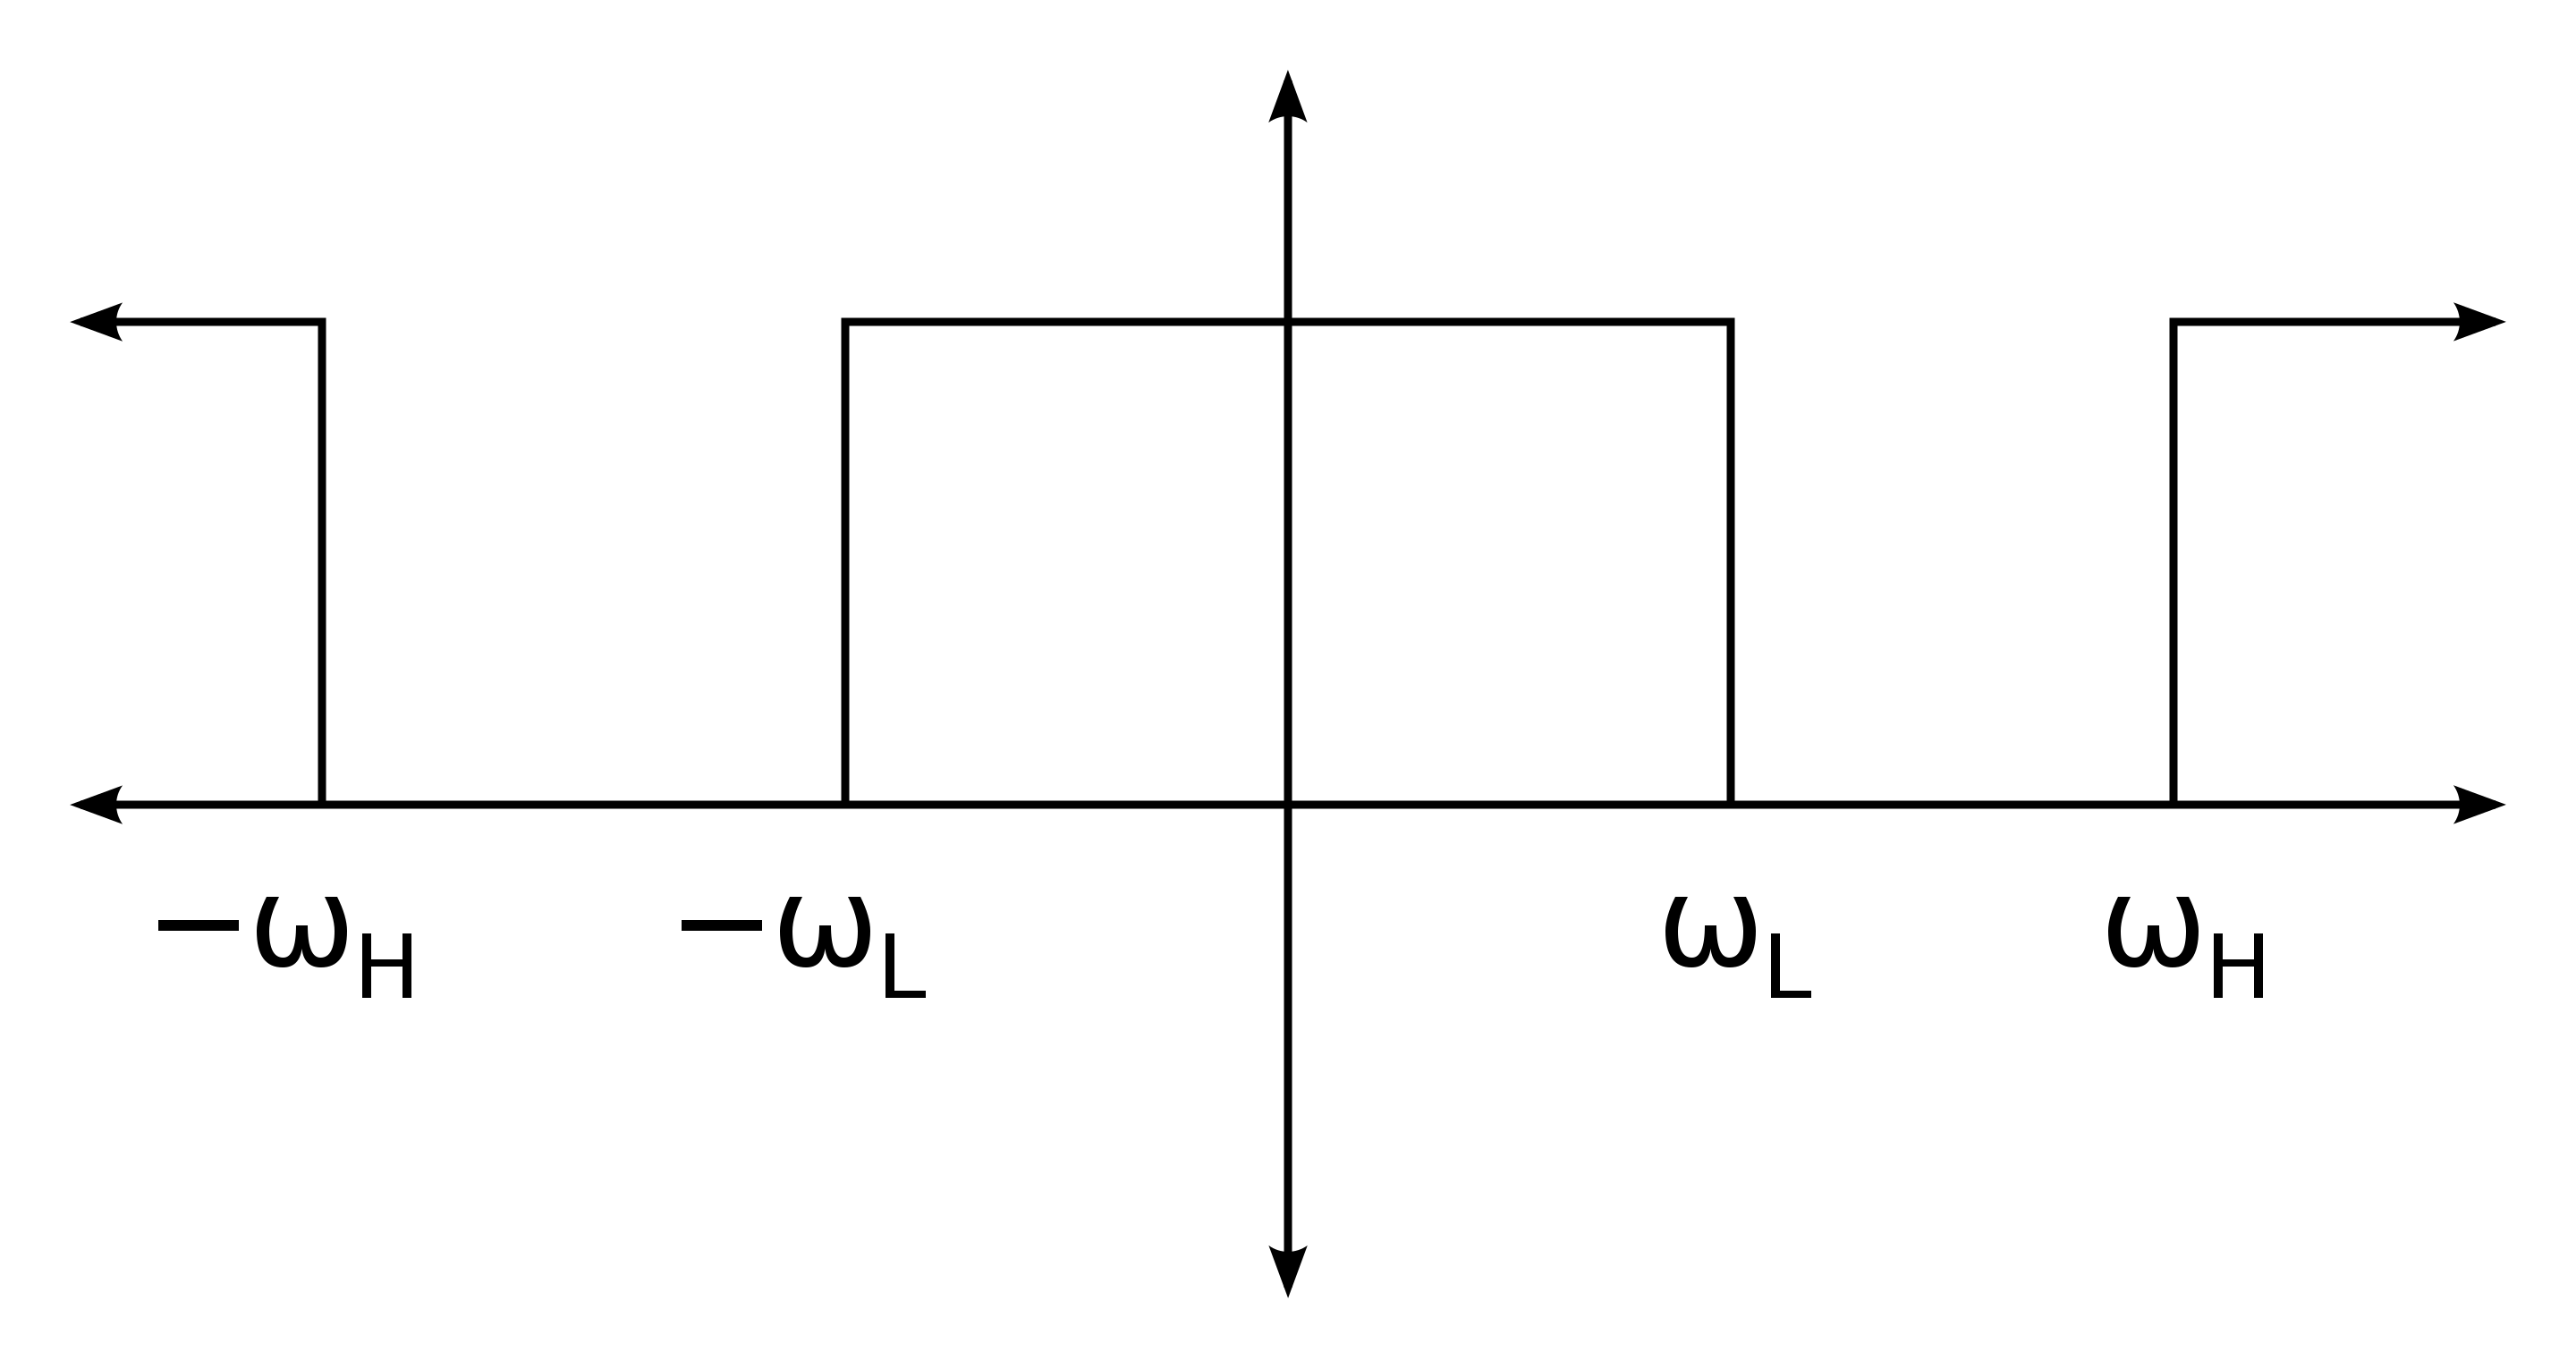
\includegraphics[width=0.6\textwidth]{images/2880px-Ideal_Band_Stop_Filter_Transfer_Function.svg.png}
    \centering
    \caption{Fourrier Transformation of the angular frequency spectrum of a bandstop filter.}
    \label{fig:bsf}
\end{figure}
\section{Experimental arrangement}

\begin{itemize}
The following materials are necessary to conduct the experiment:
    \item oscilloscope that can generate waves
    \item breadboard and jumper cables
    \item 1k$\Omega$, 200$\Omega$, 10k$\Omega$ resistors
    \item 100$\mu$F, 220$\mu$F, 47$\mu$F capacitors
    \item cables to connect the oscilloscope to the circuit
    \item one 6H inductor
\end{itemize}

The circuit has to be assembled according to the following schematic (fig. \ref{fig:schematic}). We did different measurements with the different electrical components from above. 

    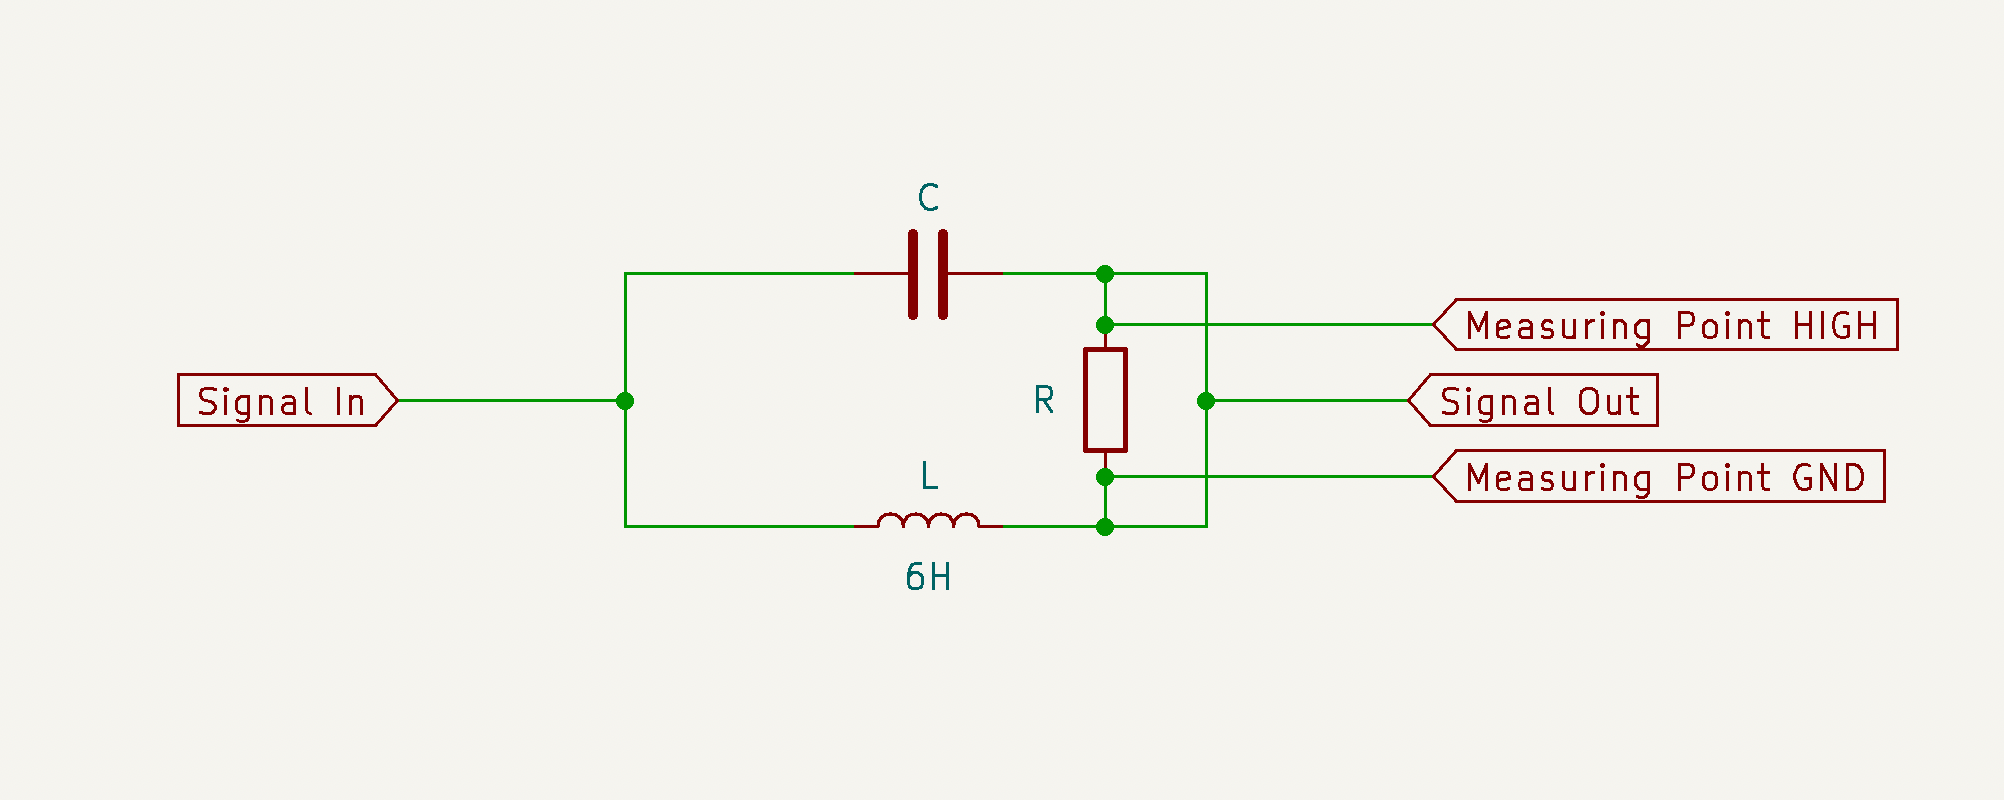
\includegraphics[width=0.8\textwidth]{images/Screenshot 2023-04-05 at 21.19.41.png}
    \centering
\begin{figure}[!ht]
    \caption{Schematic}
\end{figure}

    \label{fig:schematic}
We conducted an impulse response analysis. With this type of analysis one sends a very short electrical pulse through a system and watches how the system reacts to this signal. In LC-circuits the short electrical pulse leads to the charging of the capacitor and thus to a oscillating circuit. The oscillation is damped by a resistor so that the oscillation stops until the next pulse arrives.
\subsection{Measurement process}

\section{Analysis}

\subsection{Observations}
We could observe strange behaviour when the Measuring Point GND (see fig. \ref{fig:schematic}) was not connected to the circuit. The measured signal oscillated way more than when the pin was connectd.


\subsection{Error discussion}

    \item 
\begin{itemize}

\end{itemize}

\section{Conclusion}

\bibliographystyle{alpha}
\bibliography{sample}

\end{document}